\documentclass[11pt,a4paper,oneside]{book}

% ========== PACKAGES ==========
\usepackage[utf8]{inputenc}
\usepackage[T1]{fontenc}
\usepackage[english]{babel}
\usepackage{geometry}
\usepackage{xcolor}
\usepackage{tikz}
\usepackage{tcolorbox}
\usepackage{graphicx}
\usepackage{enumitem}
\usepackage{hyperref}
\usepackage{fancyhdr}
\usepackage{titlesec}
\usepackage{listings}
\usepackage{fontawesome5}
\usepackage{booktabs}
\usepackage{array}
\usepackage{longtable}
\usepackage{float}
\usepackage{caption}
\usepackage{subcaption}

% ========== GEOMETRY ==========
\geometry{
    a4paper,
    left=2.5cm,
    right=2.5cm,
    top=3cm,
    bottom=3cm,
    headheight=15pt
}

% ========== COLOR PALETTE ==========
\definecolor{primaryblue}{RGB}{23,54,93}
\definecolor{accentteal}{RGB}{1,210,119}
\definecolor{accentorange}{RGB}{255,159,64}
\definecolor{darkgray}{RGB}{45,45,45}
\definecolor{lightgray}{RGB}{245,245,245}
\definecolor{codebackground}{RGB}{248,249,250}
\definecolor{warningred}{RGB}{220,53,69}
\definecolor{successgreen}{RGB}{40,167,69}

% ========== HYPERLINKS ==========
\hypersetup{
    colorlinks=true,
    linkcolor=primaryblue,
    filecolor=accentteal,
    urlcolor=accentteal,
    citecolor=primaryblue,
    pdftitle={React Native Movie App - Technical Documentation},
    pdfauthor={Mausam Kar},
    pdfsubject={Mobile Application Development},
    pdfkeywords={React Native, Mobile App, TMDB, Appwrite}
}

% ========== TIKZ LIBRARIES ==========
\usetikzlibrary{shapes,arrows,positioning,shadows,decorations.pathreplacing,calc}

% ========== TCOLORBOX SETTINGS ==========
\tcbuselibrary{skins,breakable}

% Custom boxes
\newtcolorbox{definitionbox}[1]{
    colback=lightgray,
    colframe=primaryblue,
    fonttitle=\bfseries,
    title=#1,
    arc=2mm,
    boxrule=1pt,
    breakable
}

\newtcolorbox{keypoint}[1]{
    colback=accentteal!10,
    colframe=accentteal,
    fonttitle=\bfseries,
    title=\faCheckCircle\ #1,
    arc=2mm,
    boxrule=1.5pt,
    breakable
}

\newtcolorbox{notebox}{
    colback=accentorange!10,
    colframe=accentorange,
    fonttitle=\bfseries,
    title=\faExclamationTriangle\ Important Note,
    arc=2mm,
    boxrule=1.5pt,
    breakable
}

% ========== CHAPTER/SECTION STYLING ==========
\titleformat{\chapter}[display]
{\normalfont\huge\bfseries\color{primaryblue}}
{\filleft\Large\chaptertitlename\ \thechapter}
{2ex}
{\titlerule\vspace{2ex}\filleft}
[\vspace{1ex}\titlerule]

\titleformat{\section}
{\normalfont\Large\bfseries\color{primaryblue}}
{\thesection}{1em}{}

\titleformat{\subsection}
{\normalfont\large\bfseries\color{accentteal}}
{\thesubsection}{1em}{}

% ========== HEADER/FOOTER ==========
\pagestyle{fancy}
\fancyhf{}
\fancyhead[L]{\leftmark}
\fancyhead[R]{\thepage}
\fancyfoot[C]{\small\textit{React Native Movie App - Technical Documentation}}
\renewcommand{\headrulewidth}{0.5pt}
\renewcommand{\footrulewidth}{0.5pt}

% ========== CODE LISTINGS ==========
\lstdefinestyle{codestyle}{
    backgroundcolor=\color{codebackground},
    commentstyle=\color{successgreen},
    keywordstyle=\color{primaryblue}\bfseries,
    numberstyle=\tiny\color{darkgray},
    stringstyle=\color{accentorange},
    basicstyle=\ttfamily\footnotesize,
    breakatwhitespace=false,
    breaklines=true,
    captionpos=b,
    keepspaces=true,
    numbers=left,
    numbersep=5pt,
    showspaces=false,
    showstringspaces=false,
    showtabs=false,
    tabsize=2,
    frame=single,
    rulecolor=\color{darkgray}
}
\lstset{style=codestyle}

% ========== DOCUMENT START ==========
\begin{document}

% ========== TITLE PAGE ==========
\begin{titlepage}
    \begin{tikzpicture}[remember picture,overlay]
        % Background gradient
        \fill[primaryblue] (current page.south west) rectangle (current page.north east);
        
        % Accent shapes
        \fill[accentteal,opacity=0.3] (current page.north west) -- ++(0,-8) -- ++(10,0) -- cycle;
        \fill[accentorange,opacity=0.2] (current page.south east) -- ++(0,6) -- ++(-12,0) -- cycle;
        
        % Content
        \node[text width=14cm,align=center] at (current page.center) {
            {\Huge\bfseries\color{white} REACT NATIVE\\[0.3cm] MOVIE APP}\\[1cm]
            {\Large\color{accentteal} Technical Documentation \& Architecture}\\[2cm]
            {\large\color{white} A Modern Cross-Platform Mobile Application}\\
            {\large\color{white} for Movie Discovery and Analytics}\\[3cm]
            {\LARGE\bfseries\color{accentorange} Mausam Kar}\\[0.5cm]
            {\large\color{white} \today}
        };
        
        % Bottom decorative line
        \draw[accentteal,line width=2pt] ([yshift=2cm]current page.south west) -- ([yshift=2cm]current page.south east);
    \end{tikzpicture}
\end{titlepage}

% ========== TABLE OF CONTENTS ==========
\tableofcontents
\clearpage

% ========== CHAPTER 1: OVERVIEW ==========
\chapter{Project Overview}

\section{Introduction}

The React Native Movie App is a modern, cross-platform mobile application that leverages \textbf{The Movie Database (TMDB) API} to provide users with comprehensive movie information. Built with React Native and Expo, the application features a sleek user interface powered by NativeWind (TailwindCSS), real-time trending analytics through Appwrite, and smooth animations for an exceptional user experience.

\begin{keypoint}{Key Highlights}
\begin{itemize}[leftmargin=*]
    \item \textbf{Real-time Trending Movies:} Based on user search patterns and analytics
    \item \textbf{Intelligent Search:} Debounced search with automatic analytics tracking
    \item \textbf{Beautiful UI/UX:} Modern design with smooth animations and gradients
    \item \textbf{Search Analytics:} Powered by Appwrite backend database
    \item \textbf{Cross-Platform:} Native support for iOS, Android, and Web
    \item \textbf{Fast Performance:} Optimized data fetching and rendering
\end{itemize}
\end{keypoint}

\section{Application Vision}

This application represents a convergence of modern mobile development practices, cloud-based backend services, and user-centric design principles. The primary goal is to create an engaging platform where users can discover movies, explore trending content, and receive personalized recommendations based on collective user behavior.

\subsection{Target Audience}

\begin{itemize}[leftmargin=*]
    \item Movie enthusiasts seeking comprehensive information
    \item Users looking for trending and popular content
    \item Mobile-first consumers who prefer native app experiences
    \item Developers studying modern React Native architecture
\end{itemize}

\subsection{Design Philosophy}

The application follows a clean, minimal design approach while maintaining rich functionality. Every interaction is carefully crafted to feel responsive and intuitive, leveraging native animations and gesture handling to create a premium user experience.

% ========== CHAPTER 2: FEATURES ==========
\chapter{Features \& Capabilities}

\section{Core Features}

\begin{table}[H]
\centering
\small
\begin{tabular}{@{}p{4cm}p{9cm}@{}}
\toprule
\textbf{Feature} & \textbf{Description} \\
\midrule
Movie Discovery & Browse popular and latest movies from TMDB with high-quality posters and detailed information \\
\addlinespace
Advanced Search & Real-time search with debounced input for optimized API calls and reduced network traffic \\
\addlinespace
Trending Movies & Horizontal scrollable carousel displaying the most searched movies by all users \\
\addlinespace
Search Analytics & Automatically track search queries and build dynamic trending lists using Appwrite \\
\addlinespace
Movie Details & Comprehensive information including ratings, release dates, cast, and plot descriptions \\
\addlinespace
Responsive Design & Beautiful UI that adapts seamlessly to different screen sizes and orientations \\
\addlinespace
Smooth Animations & Engaging animations powered by React Native Reanimated for fluid transitions \\
\addlinespace
Tab Navigation & Intuitive bottom tab navigation for easy exploration across app sections \\
\addlinespace
Error Handling & Graceful error handling with user-friendly messages and retry mechanisms \\
\addlinespace
Loading States & Activity indicators providing clear feedback during data fetching operations \\
\bottomrule
\end{tabular}
\caption{Complete Feature Breakdown}
\end{table}

\section{User Interface Components}

\subsection{Home Screen}

The home screen serves as the primary entry point, featuring:

\begin{definitionbox}{Trending Section}
A horizontally scrollable carousel showcasing the top 5 most searched movies. This section updates dynamically based on aggregated user search behavior stored in the Appwrite database.
\end{definitionbox}

\begin{definitionbox}{Latest Movies Grid}
A vertically scrollable grid displaying popular and latest releases from TMDB. Each movie card includes poster artwork, title, and rating information.
\end{definitionbox}

\subsection{Search Screen}

The search interface provides:

\begin{itemize}[leftmargin=*]
    \item \textbf{Real-time Search Bar:} Debounced input (500ms) to optimize API calls
    \item \textbf{Results Grid:} 3-column responsive grid layout
    \item \textbf{Empty States:} Contextual messages when no results are found
    \item \textbf{Analytics Tracking:} Automatic search query logging
\end{itemize}

\subsection{Movie Detail View}

\begin{notebox}
The detailed movie view is planned for future releases and will include comprehensive information such as full cast, reviews, similar movies, and streaming availability.
\end{notebox}

% ========== CHAPTER 3: ARCHITECTURE ==========
\chapter{System Architecture}

\section{High-Level Architecture}

The application follows a layered architecture pattern with clear separation of concerns:

\begin{figure}[H]
\centering
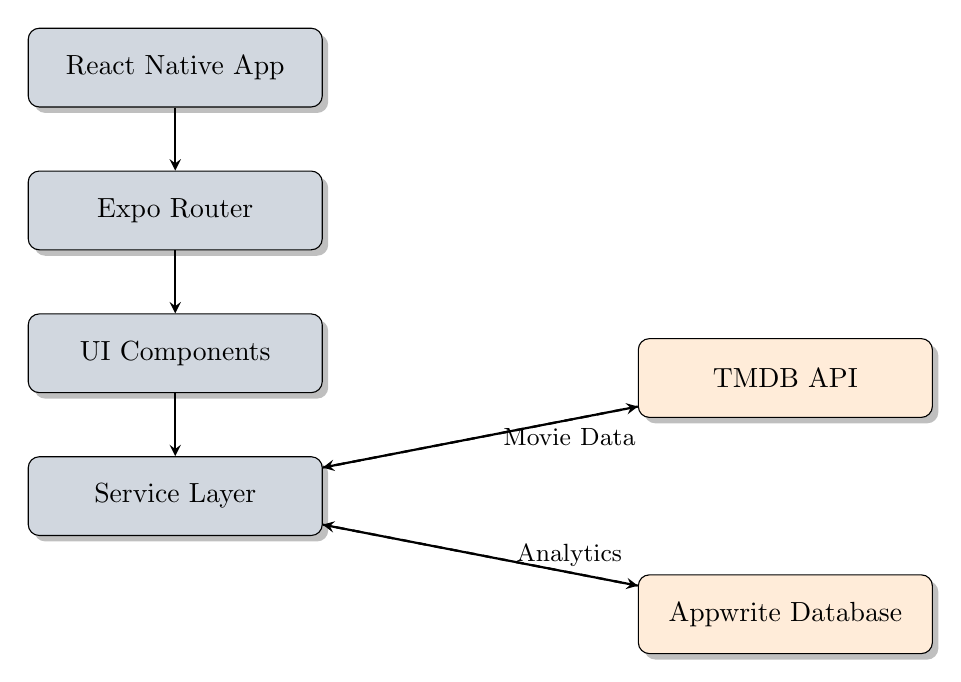
\begin{tikzpicture}[
    node distance=1.5cm,
    component/.style={rectangle, draw, fill=primaryblue!20, text width=3.5cm, text centered, rounded corners, minimum height=1cm, drop shadow},
    service/.style={rectangle, draw, fill=accentteal!20, text width=3.5cm, text centered, rounded corners, minimum height=1cm, drop shadow},
    external/.style={rectangle, draw, fill=accentorange!20, text width=3.5cm, text centered, rounded corners, minimum height=1cm, drop shadow},
    arrow/.style={->,>=stealth,thick}
]

% Mobile App Layer
\node[component] (app) {React Native App};
\node[component, below=0.8cm of app] (router) {Expo Router};
\node[component, below=0.8cm of router] (ui) {UI Components};
\node[component, below=0.8cm of ui] (service) {Service Layer};

% External Services
\node[external, right=4cm of service, yshift=1.5cm] (tmdb) {TMDB API};
\node[external, right=4cm of service, yshift=-1.5cm] (appwrite) {Appwrite Database};

% Arrows
\draw[arrow] (app) -- (router);
\draw[arrow] (router) -- (ui);
\draw[arrow] (ui) -- (service);
\draw[arrow] (service) -- (tmdb);
\draw[arrow] (service) -- (appwrite);
\draw[arrow, dashed] (tmdb) -- node[right, text width=2cm, align=center] {\small Movie Data} (service);
\draw[arrow, dashed] (appwrite) -- node[right, text width=2cm, align=center] {\small Analytics} (service);

\end{tikzpicture}
\caption{System Architecture Overview}
\end{figure}

\section{Component Breakdown}

\subsection{Mobile Application Layer}

\begin{definitionbox}{React Native Framework}
The foundation of the application, providing cross-platform capabilities and native performance. React Native enables code reuse across iOS, Android, and web platforms while maintaining native UI components.
\end{definitionbox}

\subsection{Routing \& Navigation}

\begin{definitionbox}{Expo Router}
File-based routing system that automatically generates navigation structure from the project's file hierarchy. This approach simplifies navigation management and improves maintainability.
\end{definitionbox}

\subsection{Service Layer Architecture}

The service layer acts as an abstraction between the UI and external data sources:

\begin{itemize}[leftmargin=*]
    \item \textbf{API Service:} Handles all TMDB API interactions
    \item \textbf{Appwrite Service:} Manages database operations for analytics
    \item \textbf{Custom Hooks:} Reusable data fetching logic with loading/error states
\end{itemize}

\section{External Services Integration}

\subsection{TMDB API}

The Movie Database API provides:
\begin{itemize}[leftmargin=*]
    \item Comprehensive movie information and metadata
    \item High-quality poster and backdrop images
    \item Search functionality with fuzzy matching
    \item Popular and trending movie endpoints
    \item Movie ratings and user reviews
\end{itemize}

\subsection{Appwrite Backend}

Appwrite serves as the Backend-as-a-Service (BaaS) platform for:
\begin{itemize}[leftmargin=*]
    \item Search analytics collection and storage
    \item Real-time trending data computation
    \item User authentication (future enhancement)
    \item Database operations with built-in permissions
\end{itemize}

% ========== CHAPTER 4: DATA FLOW ==========
\chapter{Application Workflow}

\section{Search Flow Process}

\begin{figure}[H]
\centering
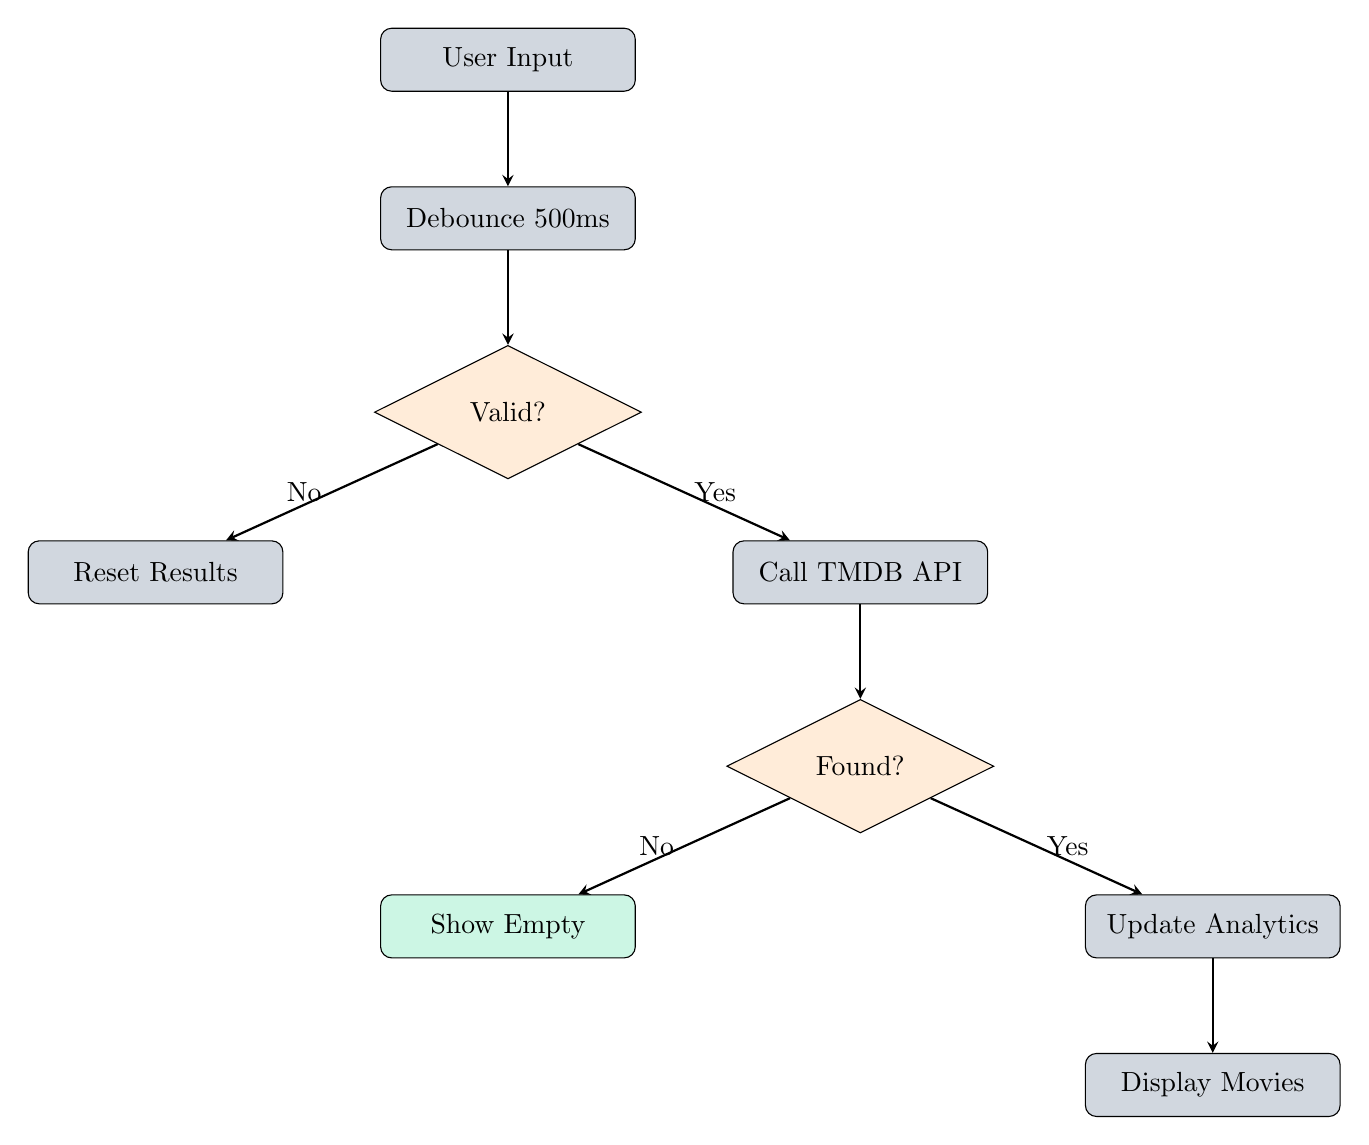
\begin{tikzpicture}[
    node distance=1.2cm and 2cm,
    process/.style={rectangle, draw, fill=primaryblue!20, text width=3cm, text centered, rounded corners, minimum height=0.8cm},
    decision/.style={diamond, draw, fill=accentorange!20, text width=2.2cm, text centered, aspect=2},
    data/.style={rectangle, draw, fill=accentteal!20, text width=3cm, text centered, rounded corners, minimum height=0.8cm},
    arrow/.style={->,>=stealth,thick}
]

\node[process] (input) {User Input};
\node[process, below=of input] (debounce) {Debounce 500ms};
\node[decision, below=of debounce] (validate) {Valid?};
\node[process, below left=of validate] (reset) {Reset Results};
\node[process, below right=of validate] (search) {Call TMDB API};
\node[decision, below=of search] (results) {Found?};
\node[data, below left=of results] (empty) {Show Empty};
\node[process, below right=of results] (update) {Update Analytics};
\node[process, below=of update] (display) {Display Movies};

\draw[arrow] (input) -- (debounce);
\draw[arrow] (debounce) -- (validate);
\draw[arrow] (validate) -- node[left] {No} (reset);
\draw[arrow] (validate) -- node[right] {Yes} (search);
\draw[arrow] (search) -- (results);
\draw[arrow] (results) -- node[left] {No} (empty);
\draw[arrow] (results) -- node[right] {Yes} (update);
\draw[arrow] (update) -- (display);

\end{tikzpicture}
\caption{Search Workflow Diagram}
\end{figure}

\section{Analytics Tracking}

\subsection{Search Count Mechanism}

When a user performs a search:

\begin{enumerate}[leftmargin=*]
    \item Query is sent to TMDB API
    \item If results are found, check Appwrite database for existing record
    \item If record exists, increment the count field
    \item If new search term, create new database entry
    \item Update trending calculations asynchronously
\end{enumerate}

\begin{keypoint}{Performance Optimization}
The analytics update happens asynchronously and doesn't block the UI. Even if the Appwrite update fails, users still receive their search results without interruption.
\end{keypoint}

\section{Data Fetching Strategy}

\subsection{Home Screen Loading}

\begin{lstlisting}[language=JavaScript, caption=Data Fetching Pattern]
useEffect(() => {
  // Fetch popular movies from TMDB
  fetchPopularMovies();
  
  // Fetch trending from Appwrite
  fetchTrendingMovies();
}, []);
\end{lstlisting}

\subsection{Caching \& Optimization}

\begin{itemize}[leftmargin=*]
    \item Search queries are debounced to reduce API calls
    \item Results are temporarily cached in component state
    \item Images are lazy-loaded and cached by React Native
    \item Network requests include proper error boundaries
\end{itemize}

% ========== CHAPTER 5: TECH STACK ==========
\chapter{Technology Stack}

\section{Core Technologies}

\begin{table}[H]
\centering
\small
\begin{tabular}{@{}llp{5cm}p{4.5cm}@{}}
\toprule
\textbf{Category} & \textbf{Technology} & \textbf{Version} & \textbf{Purpose} \\
\midrule
Framework & React Native & 0.81.5 & Cross-platform mobile development \\
\addlinespace
Runtime & Expo & 54.0.0 & Development framework and build tools \\
\addlinespace
Language & TypeScript & 5.3.3 & Type-safe JavaScript with enhanced IDE support \\
\addlinespace
Routing & Expo Router & 6.0.19 & File-based navigation system \\
\addlinespace
Styling & NativeWind & 4.1.23 & TailwindCSS for React Native \\
\addlinespace
Styling & TailwindCSS & 3.4.17 & Utility-first CSS framework \\
\addlinespace
Backend & Appwrite & 0.19.0 & Backend-as-a-Service platform \\
\addlinespace
API & TMDB API & v3 & Movie database and information \\
\addlinespace
Animations & Reanimated & 3.16.0 & High-performance animations \\
\addlinespace
Gestures & Gesture Handler & 2.28.0 & Touch gesture management \\
\addlinespace
Icons & Heroicons & 4.0.0 & Beautiful SVG icon set \\
\addlinespace
Navigation & React Navigation & 7.0.14 & Navigation infrastructure \\
\bottomrule
\end{tabular}
\caption{Complete Technology Stack}
\end{table}

\section{Development Tools}

\begin{definitionbox}{TypeScript}
Provides static type checking, enhanced IDE support, and improved code maintainability. TypeScript catches errors during development rather than runtime, significantly improving code quality.
\end{definitionbox}

\begin{definitionbox}{NativeWind}
Brings the power of TailwindCSS to React Native, enabling rapid UI development with utility classes while maintaining native performance and feel.
\end{definitionbox}

\section{Third-Party Integrations}

\subsection{The Movie Database (TMDB)}

\begin{itemize}[leftmargin=*]
    \item Industry-standard movie database with comprehensive information
    \item RESTful API with excellent documentation
    \item High-quality images and metadata
    \item Free tier suitable for development and small applications
\end{itemize}

\subsection{Appwrite Platform}

\begin{itemize}[leftmargin=*]
    \item Open-source Backend-as-a-Service
    \item Built-in database with real-time capabilities
    \item Fine-grained permission system
    \item Authentication services (for future implementation)
    \item Cloud or self-hosted deployment options
\end{itemize}

% ========== CHAPTER 6: PROJECT STRUCTURE ==========
\chapter{Project Structure}

\section{Directory Organization}

\begin{lstlisting}[language=bash, caption=Project Directory Structure, numbers=none]
react-native-movie-app/
|
|-- app/                    # Application screens and routes
|   |-- (tabs)/            # Tab-based navigation screens
|   |   |-- index.tsx      # Home screen
|   |   `-- search.tsx     # Search screen
|   |-- movie/             # Movie detail screens
|   |   `-- [id].tsx       # Dynamic movie detail page
|   |-- _layout.tsx        # Root layout configuration
|   `-- globals.css        # Global styles
|
|-- components/            # Reusable UI components
|   |-- MovieCard.tsx      # Movie grid card
|   |-- SearchBar.tsx      # Search input
|   `-- TrendingCard.tsx   # Trending carousel card
|
|-- services/              # Business logic and API
|   |-- api.ts            # TMDB API integration
|   |-- appwrite.ts       # Appwrite operations
|   `-- usefetch.ts       # Custom data fetching hook
|
|-- constants/             # App constants
|   |-- icons.ts          # Icon exports
|   `-- images.ts         # Image exports
|
|-- interfaces/            # TypeScript definitions
|-- types/                # Additional type declarations
|-- assets/               # Static assets
|-- .env                  # Environment variables
|-- app.json              # Expo configuration
|-- package.json          # Dependencies
|-- tailwind.config.js    # TailwindCSS config
`-- tsconfig.json         # TypeScript config
\end{lstlisting}

\section{Key Files Explained}

\subsection{Application Routes (app/ directory)}

\begin{definitionbox}{File-Based Routing}
Expo Router uses the file system as the API for routing. Each file in the \texttt{app/} directory automatically becomes a route in the application.
\end{definitionbox}

\begin{itemize}[leftmargin=*]
    \item \texttt{(tabs)/index.tsx}: Home screen with trending and popular movies
    \item \texttt{(tabs)/search.tsx}: Search interface with analytics
    \item \texttt{movie/[id].tsx}: Dynamic route for individual movie details
    \item \texttt{\_layout.tsx}: Root layout defining app-wide navigation structure
\end{itemize}

\subsection{Services Layer}

\begin{definitionbox}{api.ts}
Handles all TMDB API interactions including search, popular movies, and movie details. Includes error handling and response transformation.
\end{definitionbox}

\begin{definitionbox}{appwrite.ts}
Manages Appwrite database operations for search analytics, including creating, reading, and updating search count records.
\end{definitionbox}

\begin{definitionbox}{usefetch.ts}
Custom React hook providing reusable data fetching logic with loading states, error handling, and automatic cleanup.
\end{definitionbox}

% ========== CHAPTER 7: INSTALLATION ==========
\chapter{Installation \& Setup}

\section{Prerequisites}

\begin{keypoint}{System Requirements}
\begin{itemize}[leftmargin=*]
    \item \textbf{Node.js:} Version 18 or higher
    \item \textbf{Package Manager:} npm or yarn
    \item \textbf{Expo CLI:} Installed globally
    \item \textbf{Git:} For version control
    \item \textbf{TMDB Account:} For API access
    \item \textbf{Appwrite Account:} For backend services
\end{itemize}
\end{keypoint}

\subsection{Platform-Specific Requirements}

\begin{table}[H]
\centering
\begin{tabular}{@{}llp{7cm}@{}}
\toprule
\textbf{Platform} & \textbf{Tool} & \textbf{Purpose} \\
\midrule
iOS & Xcode & iOS simulator and build tools (macOS only) \\
Android & Android Studio & Android SDK and emulator \\
Mobile Testing & Expo Go App & Test on physical devices without building \\
\bottomrule
\end{tabular}
\end{table}

\section{Step-by-Step Installation}

\subsection{1. Clone Repository}

\begin{lstlisting}[language=bash, caption=Clone the Project]
git clone https://github.com/yourusername/react-native-movie-app.git
cd react-native-movie-app
\end{lstlisting}

\subsection{2. Install Dependencies}

\begin{lstlisting}[language=bash, caption=Install Node Packages]
npm install
# Alternative: yarn install
\end{lstlisting}

\subsection{3. Environment Configuration}

Create a \texttt{.env} file in the project root:

\begin{lstlisting}[language=bash, caption=Environment Variables, numbers=none]
EXPO_PUBLIC_MOVIE_API_KEY=your_tmdb_api_key_here
EXPO_PUBLIC_APPWRITE_PROJECT_ID=your_project_id
EXPO_PUBLIC_APPWRITE_DATABASE_ID=your_database_id
EXPO_PUBLIC_APPWRITE_COLLECTION_ID=your_collection_id
EXPO_PUBLIC_APPWRITE_ENDPOINT=https://cloud.appwrite.io/v1
\end{lstlisting}

\section{TMDB API Setup}

\subsection{Obtaining API Key}

\begin{enumerate}[leftmargin=*]
    \item Visit \href{https://www.themoviedb.org/}{TMDB Website}
    \item Create an account or log in
    \item Navigate to: \textbf{Settings} → \textbf{API} → \textbf{Request API Key}
    \item Select ``Developer'' option
    \item Complete the application form
    \item Copy your \textbf{API Read Access Token (v4 auth)}
    \item Add to \texttt{.env} file as \texttt{EXPO\_PUBLIC\_MOVIE\_API\_KEY}
\end{enumerate}

\begin{notebox}
Use the v4 Bearer token, not the v3 API key. The v4 token provides better security and functionality.
\end{notebox}

\section{Appwrite Backend Configuration}

\subsection{Project Setup}

\begin{enumerate}[leftmargin=*]
    \item Go to \href{https://cloud.appwrite.io/}{Appwrite Console}
    \item Create a new project
    \item Copy the \textbf{Project ID}
    \item Add to \texttt{.env} file
\end{enumerate}

\subsection{Database Creation}

\begin{enumerate}[leftmargin=*]
    \item Navigate to \textbf{Databases} section
    \item Click \textbf{``Create Database''}
    \item Name it (e.g., ``MovieAppDB'')
    \item Copy the \textbf{Database ID}
    \item Add to \texttt{.env} file
\end{enumerate}

\subsection{Collection Configuration}

\begin{enumerate}[leftmargin=*]
    \item Inside your database, click \textbf{``Create Collection''}
    \item Name it \textbf{``movies''}
    \item Copy the \textbf{Collection ID}
    \item Add to \texttt{.env} file
\end{enumerate}

\subsection{Collection Attributes}

Add the following attributes to your collection:

\begin{table}[H]
\centering
\begin{tabular}{@{}llcc@{}}
\toprule
\textbf{Attribute} & \textbf{Type} & \textbf{Size} & \textbf{Required} \\
\midrule
searchTerm & String & 255 & Yes \\
movie\_id & Integer & --- & Yes \\
title & String & 500 & Yes \\
count & Integer & --- & Yes \\
poster\_url & String & 1000 & No \\
\bottomrule
\end{tabular}
\caption{Appwrite Collection Schema}
\end{table}

\subsection{Permissions Configuration}

\begin{keypoint}{Required Permissions}
Set the following permissions for the \textbf{``Any''} role:
\begin{itemize}[leftmargin=*]
    \item \textbf{Read:} Allow users to view trending data
    \item \textbf{Create:} Allow creating new search entries
    \item \textbf{Update:} Allow incrementing search counts
\end{itemize}
\end{keypoint}

% ========== CHAPTER 8: USAGE ==========
\chapter{Running the Application}

\section{Development Server}

\subsection{Start Expo Development Server}

\begin{lstlisting}[language=bash, caption=Start Development Server]
npm start
# Alternative: expo start
\end{lstlisting}

This launches the Expo development server and displays a QR code in the terminal.

\section{Platform-Specific Execution}

\subsection{iOS Development}

\begin{lstlisting}[language=bash, caption=Run on iOS Simulator]
npm run ios
\end{lstlisting}

\begin{notebox}
iOS development requires macOS with Xcode installed. The first build may take several minutes.
\end{notebox}

\subsection{Android Development}

\begin{lstlisting}[language=bash, caption=Run on Android Emulator]
npm run android
\end{lstlisting}

Ensure Android Studio is installed and an emulator is running.

\subsection{Web Development}

\begin{lstlisting}[language=bash, caption=Run in Web Browser]
npm run web
\end{lstlisting}

Opens the application in your default web browser.

\section{Testing on Physical Devices}

\subsection{Using Expo Go}

\begin{enumerate}[leftmargin=*]
    \item Install \textbf{Expo Go} from App Store (iOS) or Play Store (Android)
    \item Start the development server: \texttt{npm start}
    \item Scan the QR code with:
    \begin{itemize}
        \item iOS: Camera app
        \item Android: Expo Go app
    \end{itemize}
    \item Application loads automatically on your device
\end{enumerate}

\begin{keypoint}{Live Reload}
Changes to your code automatically reload in Expo Go, enabling rapid development and testing.
\end{keypoint}

% ========== CHAPTER 9: FUTURE ROADMAP ==========
\chapter{Future Roadmap}

\section{Planned Enhancements}

\subsection{Video Streaming \& Downloads}

\begin{table}[H]
\centering
\small
\begin{tabular}{@{}p{4.5cm}p{7cm}c@{}}
\toprule
\textbf{Feature} & \textbf{Description} & \textbf{Status} \\
\midrule
Movie Streaming & Stream full-length movies with adaptive quality & Planned \\
Web Series Support & Browse and stream complete series with episode tracking & Planned \\
Offline Downloads & Download content for offline viewing & Planned \\
Multi-Quality Options & Choose from 480p, 720p, 1080p, 4K & Planned \\
Resume Playback & Continue from last watched position & Planned \\
Subtitle Support & Multi-language subtitle integration & Planned \\
Watch History & Track viewing progress and history & Planned \\
\bottomrule
\end{tabular}
\caption{Upcoming Features}
\end{table}

\subsection{Amazon S3 Integration}

The streaming functionality will leverage \textbf{Amazon S3} for media storage with \textbf{CloudFront} for global content delivery.

\begin{figure}[H]
\centering
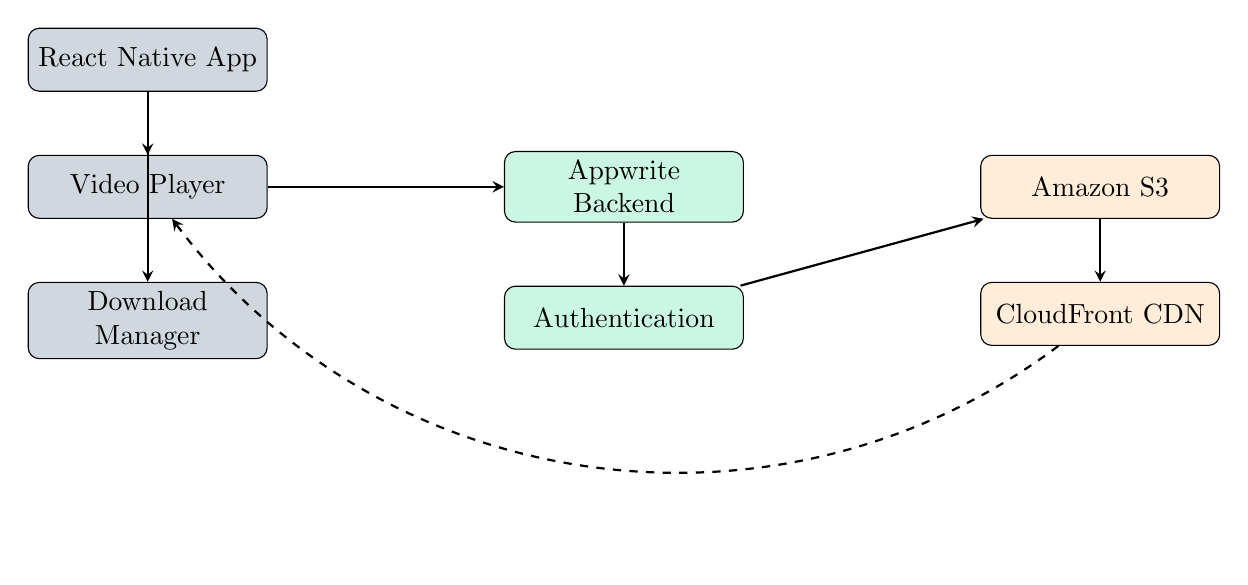
\begin{tikzpicture}[
    node distance=1.5cm,
    app/.style={rectangle, draw, fill=primaryblue!20, text width=2.8cm, text centered, rounded corners, minimum height=0.8cm},
    backend/.style={rectangle, draw, fill=accentteal!20, text width=2.8cm, text centered, rounded corners, minimum height=0.8cm},
    aws/.style={rectangle, draw, fill=accentorange!20, text width=2.8cm, text centered, rounded corners, minimum height=0.8cm},
    arrow/.style={->,>=stealth,thick}
]

\node[app] (rnapp) {React Native App};
\node[app, below=0.8cm of rnapp] (player) {Video Player};
\node[app, below=0.8cm of player] (download) {Download Manager};

\node[backend, right=3cm of player] (appwrite) {Appwrite Backend};
\node[backend, below=0.8cm of appwrite] (auth) {Authentication};

\node[aws, right=3cm of appwrite] (s3) {Amazon S3};
\node[aws, below=0.8cm of s3] (cloudfront) {CloudFront CDN};

\draw[arrow] (rnapp) -- (player);
\draw[arrow] (rnapp) -- (download);
\draw[arrow] (player) -- (appwrite);
\draw[arrow] (appwrite) -- (auth);
\draw[arrow] (auth) -- (s3);
\draw[arrow] (s3) -- (cloudfront);
\draw[arrow, dashed] (cloudfront) to [bend left=45] (player);

\end{tikzpicture}
\caption{AWS Integration Architecture}
\end{figure}

\section{Implementation Phases}

\subsection{Phase 1: Basic Streaming (Q1 2026)}

\begin{itemize}[leftmargin=*]
    \item Set up Amazon S3 buckets for video storage
    \item Configure CloudFront distribution
    \item Implement basic video player with playback controls
    \item Add authentication and presigned URL generation
    \item Support for 720p streaming quality
\end{itemize}

\subsection{Phase 2: Advanced Features (Q2 2026)}

\begin{itemize}[leftmargin=*]
    \item Multi-quality streaming (480p, 720p, 1080p, 4K)
    \item Download functionality with progress tracking
    \item Resume playback from last position
    \item Multi-language subtitle support
    \item Watch history and continue watching features
\end{itemize}

\subsection{Phase 3: Web Series Integration (Q3 2026)}

\begin{itemize}[leftmargin=*]
    \item Web series browsing and discovery
    \item Episode listing and navigation
    \item Season management system
    \item Auto-play next episode (binge-watching)
    \item Series progress tracking across devices
\end{itemize}

\subsection{Phase 4: Optimization (Q4 2026)}

\begin{itemize}[leftmargin=*]
    \item Adaptive bitrate streaming based on network
    \item Offline mode improvements
    \item Picture-in-Picture (PiP) support
    \item Chromecast/AirPlay integration
    \item AI-powered recommendations
\end{itemize}

\section{Additional Planned Features}

\begin{definitionbox}{Watchlist \& Favorites}
Users will be able to create personalized watchlists, mark favorites, and receive notifications when new content is added.
\end{definitionbox}

\begin{definitionbox}{Social Features}
Share favorite movies, write reviews, and connect with friends to see what they're watching.
\end{definitionbox}

\begin{definitionbox}{Personalized Recommendations}
AI-powered content suggestions based on viewing history, ratings, and user preferences.
\end{definitionbox}

\begin{definitionbox}{Parental Controls}
Content filtering, age restrictions, and PIN-protected profiles for family safety.
\end{definitionbox}

% ========== CHAPTER 10: TROUBLESHOOTING ==========
\chapter{Troubleshooting \& Support}

\section{Common Issues}

\begin{table}[H]
\centering
\small
\begin{tabular}{@{}p{5cm}p{7.5cm}@{}}
\toprule
\textbf{Issue} & \textbf{Solution} \\
\midrule
Metro bundler error & Clear cache: \texttt{npx expo start -c} \\
\addlinespace
Reanimated plugin errors & Ensure \texttt{babel.config.js} includes reanimated plugin \\
\addlinespace
Appwrite 401 unauthorized & Check collection permissions allow Any role to Read/Create/Update \\
\addlinespace
TMDB API errors & Verify API key is correct and uses Bearer token format \\
\addlinespace
Environment variables not loading & Restart development server after changing \texttt{.env} \\
\addlinespace
iOS build failures & Run \texttt{pod install} in the ios/ directory \\
\addlinespace
Android build failures & Clean gradle cache: \texttt{./gradlew clean} \\
\bottomrule
\end{tabular}
\caption{Troubleshooting Guide}
\end{table}

\section{Cache Clearing}

\subsection{Complete Cache Reset}

\begin{lstlisting}[language=bash, caption=Clear All Caches]
# Clear Expo cache
npx expo start -c

# Clear npm cache
npm cache clean --force

# Clear watchman (macOS/Linux)
watchman watch-del-all

# Reinstall dependencies
rm -rf node_modules package-lock.json
npm install
\end{lstlisting}

\section{Getting Help}

\subsection{Resources}

\begin{itemize}[leftmargin=*]
    \item \textbf{GitHub Issues:} Report bugs and request features
    \item \textbf{Discussions:} Ask questions and share ideas
    \item \textbf{Documentation:} Comprehensive guides and API references
    \item \textbf{Community:} Active React Native and Expo communities
\end{itemize}

% ========== CHAPTER 11: CONTRIBUTING ==========
\chapter{Contributing Guidelines}

\section{How to Contribute}

\subsection{Contribution Workflow}

\begin{enumerate}[leftmargin=*]
    \item \textbf{Fork the repository} on GitHub
    \item \textbf{Create a feature branch:} \texttt{git checkout -b feature/YourFeature}
    \item \textbf{Make your changes} with clear, descriptive commits
    \item \textbf{Write tests} for new functionality
    \item \textbf{Commit changes:} \texttt{git commit -m 'Add YourFeature'}
    \item \textbf{Push to branch:} \texttt{git push origin feature/YourFeature}
    \item \textbf{Open a Pull Request} with detailed description
\end{enumerate}

\section{Code Style Guidelines}

\begin{keypoint}{Best Practices}
\begin{itemize}[leftmargin=*]
    \item Use \textbf{TypeScript} for all new code
    \item Follow \textbf{Expo} and \textbf{React Native} conventions
    \item Prefer \textbf{functional components} with hooks
    \item Keep components \textbf{small and focused}
    \item Add \textbf{meaningful comments} for complex logic
    \item Use \textbf{descriptive variable names}
    \item Write \textbf{self-documenting code}
\end{itemize}
\end{keypoint}

\subsection{TypeScript Standards}

\begin{itemize}[leftmargin=*]
    \item Define explicit types for all function parameters
    \item Use interfaces for object shapes
    \item Avoid \texttt{any} type; use \texttt{unknown} when necessary
    \item Leverage type inference where appropriate
\end{itemize}

% ========== CHAPTER 12: CONCLUSION ==========
\chapter{Conclusion}

\section{Project Summary}

The React Native Movie App represents a modern approach to cross-platform mobile development, combining powerful technologies like React Native, Expo, and cloud-based backend services. The application demonstrates best practices in:

\begin{itemize}[leftmargin=*]
    \item Clean architecture with separation of concerns
    \item Type-safe development with TypeScript
    \item Modern UI design with NativeWind
    \item Real-time analytics and trending calculations
    \item Efficient data fetching and caching strategies
\end{itemize}

\section{Key Takeaways}

\begin{definitionbox}{Architecture Excellence}
The layered architecture ensures maintainability, scalability, and clear separation between UI, business logic, and data layers.
\end{definitionbox}

\begin{definitionbox}{User Experience}
Every interaction is designed to feel responsive and intuitive, with smooth animations and helpful loading states.
\end{definitionbox}

\begin{definitionbox}{Future-Ready}
The application is designed to accommodate future enhancements including video streaming, user accounts, and advanced personalization.
\end{definitionbox}

\section{Acknowledgments}

Special thanks to:

\begin{itemize}[leftmargin=*]
    \item \textbf{The Movie Database (TMDB)} for comprehensive movie data
    \item \textbf{Appwrite} for the excellent Backend-as-a-Service platform
    \item \textbf{Expo} for simplifying React Native development
    \item \textbf{NativeWind} for bringing TailwindCSS to React Native
    \item \textbf{React Native Community} for the amazing ecosystem
\end{itemize}

\vfill

\begin{center}
\Large
\textbf{Made with} \textcolor{warningred}{\faHeart} \textbf{using React Native \& Expo}

\vspace{1cm}

\textit{Star the repository if you find it helpful!}
\end{center}

\end{document}
